
%% bare_conf.tex
%% V1.4b
%% 2015/08/26
%% by Michael Shell
%% See:
%% http://www.michaelshell.org/
%% for current contact information.
%%
%% This is a skeleton file demonstrating the use of IEEEtran.cls
%% (requires IEEEtran.cls version 1.8b or later) with an IEEE
%% conference paper.
%%
%% Support sites:
%% http://www.michaelshell.org/tex/ieeetran/
%% http://www.ctan.org/pkg/ieeetran
%% and
%% http://www.ieee.org/

%%*************************************************************************
%% Legal Notice:
%% This code is offered as-is without any warranty either expressed or
%% implied; without even the implied warranty of MERCHANTABILITY or
%% FITNESS FOR A PARTICULAR PURPOSE! 
%% User assumes all risk.
%% In no event shall the IEEE or any contributor to this code be liable for
%% any damages or losses, including, but not limited to, incidental,
%% consequential, or any other damages, resulting from the use or misuse
%% of any information contained here.
%%
%% All comments are the opinions of their respective authors and are not
%% necessarily endorsed by the IEEE.
%%
%% This work is distributed under the LaTeX Project Public License (LPPL)
%% ( http://www.latex-project.org/ ) version 1.3, and may be freely used,
%% distributed and modified. A copy of the LPPL, version 1.3, is included
%% in the base LaTeX documentation of all distributions of LaTeX released
%% 2003/12/01 or later.
%% Retain all contribution notices and credits.
%% ** Modified files should be clearly indicated as such, including  **
%% ** renaming them and changing author support contact information. **
%%*************************************************************************


% *** Authors should verify (and, if needed, correct) their LaTeX system  ***
% *** with the testflow diagnostic prior to trusting their LaTeX platform ***
% *** with production work. The IEEE's font choices and paper sizes can   ***
% *** trigger bugs that do not appear when using other class files.       ***                          ***
% The testflow support page is at:
% http://www.michaelshell.org/tex/testflow/



\documentclass[conference]{IEEEtran}
% Some Computer Society conferences also require the compsoc mode option,
% but others use the standard conference format.
%
% If IEEEtran.cls has not been installed into the LaTeX system files,
% manually specify the path to it like:
% \documentclass[conference]{../sty/IEEEtran}





% Some very useful LaTeX packages include:
% (uncomment the ones you want to load)


% *** MISC UTILITY PACKAGES ***
%
%\usepackage{ifpdf}
% Heiko Oberdiek's ifpdf.sty is very useful if you need conditional
% compilation based on whether the output is pdf or dvi.
% usage:
% \ifpdf
%   % pdf code
% \else
%   % dvi code
% \fi
% The latest version of ifpdf.sty can be obtained from:
% http://www.ctan.org/pkg/ifpdf
% Also, note that IEEEtran.cls V1.7 and later provides a builtin
% \ifCLASSINFOpdf conditional that works the same way.
% When switching from latex to pdflatex and vice-versa, the compiler may
% have to be run twice to clear warning/error messages.






% *** CITATION PACKAGES ***
%
%\usepackage{cite}
% cite.sty was written by Donald Arseneau
% V1.6 and later of IEEEtran pre-defines the format of the cite.sty package
% \cite{} output to follow that of the IEEE. Loading the cite package will
% result in citation numbers being automatically sorted and properly
% "compressed/ranged". e.g., [1], [9], [2], [7], [5], [6] without using
% cite.sty will become [1], [2], [5]--[7], [9] using cite.sty. cite.sty's
% \cite will automatically add leading space, if needed. Use cite.sty's
% noadjust option (cite.sty V3.8 and later) if you want to turn this off
% such as if a citation ever needs to be enclosed in parenthesis.
% cite.sty is already installed on most LaTeX systems. Be sure and use
% version 5.0 (2009-03-20) and later if using hyperref.sty.
% The latest version can be obtained at:
% http://www.ctan.org/pkg/cite
% The documentation is contained in the cite.sty file itself.






% *** GRAPHICS RELATED PACKAGES ***
%
\usepackage{graphicx}
\ifCLASSINFOpdf
  % \usepackage[pdftex]{graphicx}
  % declare the path(s) where your graphic files are
  % \graphicspath{{../pdf/}{../jpeg/}}
  % and their extensions so you won't have to specify these with
  % every instance of \includegraphics
  % \DeclareGraphicsExtensions{.pdf,.jpeg,.png}
\else
  % or other class option (dvipsone, dvipdf, if not using dvips). graphicx
  % will default to the driver specified in the system graphics.cfg if no
  % driver is specified.
  % \usepackage[dvips]{graphicx}
  % declare the path(s) where your graphic files are
  % \graphicspath{{../eps/}}
  % and their extensions so you won't have to specify these with
  % every instance of \includegraphics
  % \DeclareGraphicsExtensions{.eps}
\fi
% graphicx was written by David Carlisle and Sebastian Rahtz. It is
% required if you want graphics, photos, etc. graphicx.sty is already
% installed on most LaTeX systems. The latest version and documentation
% can be obtained at: 
% http://www.ctan.org/pkg/graphicx
% Another good source of documentation is "Using Imported Graphics in
% LaTeX2e" by Keith Reckdahl which can be found at:
% http://www.ctan.org/pkg/epslatex
%
% latex, and pdflatex in dvi mode, support graphics in encapsulated
% postscript (.eps) format. pdflatex in pdf mode supports graphics
% in .pdf, .jpeg, .png and .mps (metapost) formats. Users should ensure
% that all non-photo figures use a vector format (.eps, .pdf, .mps) and
% not a bitmapped formats (.jpeg, .png). The IEEE frowns on bitmapped formats
% which can result in "jaggedy"/blurry rendering of lines and letters as
% well as large increases in file sizes.
%
% You can find documentation about the pdfTeX application at:
% http://www.tug.org/applications/pdftex





% *** MATH PACKAGES ***
%
%\usepackage{amsmath}
% A popular package from the American Mathematical Society that provides
% many useful and powerful commands for dealing with mathematics.
%
% Note that the amsmath package sets \interdisplaylinepenalty to 10000
% thus preventing page breaks from occurring within multiline equations. Use:
%\interdisplaylinepenalty=2500
% after loading amsmath to restore such page breaks as IEEEtran.cls normally
% does. amsmath.sty is already installed on most LaTeX systems. The latest
% version and documentation can be obtained at:
% http://www.ctan.org/pkg/amsmath





% *** SPECIALIZED LIST PACKAGES ***
%
%\usepackage{algorithmic}
% algorithmic.sty was written by Peter Williams and Rogerio Brito.
% This package provides an algorithmic environment fo describing algorithms.
% You can use the algorithmic environment in-text or within a figure
% environment to provide for a floating algorithm. Do NOT use the algorithm
% floating environment provided by algorithm.sty (by the same authors) or
% algorithm2e.sty (by Christophe Fiorio) as the IEEE does not use dedicated
% algorithm float types and packages that provide these will not provide
% correct IEEE style captions. The latest version and documentation of
% algorithmic.sty can be obtained at:
% http://www.ctan.org/pkg/algorithms
% Also of interest may be the (relatively newer and more customizable)
% algorithmicx.sty package by Szasz Janos:
% http://www.ctan.org/pkg/algorithmicx




% *** ALIGNMENT PACKAGES ***
%
%\usepackage{array}
% Frank Mittelbach's and David Carlisle's array.sty patches and improves
% the standard LaTeX2e array and tabular environments to provide better
% appearance and additional user controls. As the default LaTeX2e table
% generation code is lacking to the point of almost being broken with
% respect to the quality of the end results, all users are strongly
% advised to use an enhanced (at the very least that provided by array.sty)
% set of table tools. array.sty is already installed on most systems. The
% latest version and documentation can be obtained at:
% http://www.ctan.org/pkg/array


% IEEEtran contains the IEEEeqnarray family of commands that can be used to
% generate multiline equations as well as matrices, tables, etc., of high
% quality.




% *** SUBFIGURE PACKAGES ***
%\ifCLASSOPTIONcompsoc
%  \usepackage[caption=false,font=normalsize,labelfont=sf,textfont=sf]{subfig}
%\else
%  \usepackage[caption=false,font=footnotesize]{subfig}
%\fi
% subfig.sty, written by Steven Douglas Cochran, is the modern replacement
% for subfigure.sty, the latter of which is no longer maintained and is
% incompatible with some LaTeX packages including fixltx2e. However,
% subfig.sty requires and automatically loads Axel Sommerfeldt's caption.sty
% which will override IEEEtran.cls' handling of captions and this will result
% in non-IEEE style figure/table captions. To prevent this problem, be sure
% and invoke subfig.sty's "caption=false" package option (available since
% subfig.sty version 1.3, 2005/06/28) as this is will preserve IEEEtran.cls
% handling of captions.
% Note that the Computer Society format requires a larger sans serif font
% than the serif footnote size font used in traditional IEEE formatting
% and thus the need to invoke different subfig.sty package options depending
% on whether compsoc mode has been enabled.
%
% The latest version and documentation of subfig.sty can be obtained at:
% http://www.ctan.org/pkg/subfig




% *** FLOAT PACKAGES ***
%
%\usepackage{fixltx2e}
% fixltx2e, the successor to the earlier fix2col.sty, was written by
% Frank Mittelbach and David Carlisle. This package corrects a few problems
% in the LaTeX2e kernel, the most notable of which is that in current
% LaTeX2e releases, the ordering of single and double column floats is not
% guaranteed to be preserved. Thus, an unpatched LaTeX2e can allow a
% single column figure to be placed prior to an earlier double column
% figure.
% Be aware that LaTeX2e kernels dated 2015 and later have fixltx2e.sty's
% corrections already built into the system in which case a warning will
% be issued if an attempt is made to load fixltx2e.sty as it is no longer
% needed.
% The latest version and documentation can be found at:
% http://www.ctan.org/pkg/fixltx2e


%\usepackage{stfloats}
% stfloats.sty was written by Sigitas Tolusis. This package gives LaTeX2e
% the ability to do double column floats at the bottom of the page as well
% as the top. (e.g., "\begin{figure*}[!b]" is not normally possible in
% LaTeX2e). It also provides a command:
%\fnbelowfloat
% to enable the placement of footnotes below bottom floats (the standard
% LaTeX2e kernel puts them above bottom floats). This is an invasive package
% which rewrites many portions of the LaTeX2e float routines. It may not work
% with other packages that modify the LaTeX2e float routines. The latest
% version and documentation can be obtained at:
% http://www.ctan.org/pkg/stfloats
% Do not use the stfloats baselinefloat ability as the IEEE does not allow
% \baselineskip to stretch. Authors submitting work to the IEEE should note
% that the IEEE rarely uses double column equations and that authors should try
% to avoid such use. Do not be tempted to use the cuted.sty or midfloat.sty
% packages (also by Sigitas Tolusis) as the IEEE does not format its papers in
% such ways.
% Do not attempt to use stfloats with fixltx2e as they are incompatible.
% Instead, use Morten Hogholm'a dblfloatfix which combines the features
% of both fixltx2e and stfloats:
%
% \usepackage{dblfloatfix}
% The latest version can be found at:
% http://www.ctan.org/pkg/dblfloatfix




% *** PDF, URL AND HYPERLINK PACKAGES ***
%
%\usepackage{url}
% url.sty was written by Donald Arseneau. It provides better support for
% handling and breaking URLs. url.sty is already installed on most LaTeX
% systems. The latest version and documentation can be obtained at:
% http://www.ctan.org/pkg/url
% Basically, \url{my_url_here}.
\usepackage{url}



% *** Do not adjust lengths that control margins, column widths, etc. ***
% *** Do not use packages that alter fonts (such as pslatex).         ***
% There should be no need to do such things with IEEEtran.cls V1.6 and later.
% (Unless specifically asked to do so by the journal or conference you plan
% to submit to, of course. )


% correct bad hyphenation here
\hyphenation{op-tical net-works semi-conduc-tor}

% *** Algorithm and Algorithmic packages ***
\usepackage{algorithm, algorithmic}

% *** footnote package *** %
\usepackage{footnote}

% *** euqation packages *** %
\usepackage{amsmath}


\begin{document}
%
% paper title
% Titles are generally capitalized except for words such as a, an, and, as,
% at, but, by, for, in, nor, of, on, or, the, to and up, which are usually
% not capitalized unless they are the first or last word of the title.
% Linebreaks \\ can be used within to get better formatting as desired.
% Do not put math or special symbols in the title.
\title{Evolving Deep Convolutional Neural Networks by Particle Swarm Optimization for Image Classification}


% author names and affiliations
% use a multiple column layout for up to three different
% affiliations
\author{
\IEEEauthorblockN{Bin Wang, Mengjie Zhang, Bing Xue, Yanan Sun, Harith Al-Sahaf}
\IEEEauthorblockA{School of Engineering\\ and Computer Science\\
	Victoria University of Wellington\\
	Kelburn, Wellington 6012}
}


% conference papers do not typically use \thanks and this command
% is locked out in conference mode. If really needed, such as for
% the acknowledgment of grants, issue a \IEEEoverridecommandlockouts
% after \documentclass

% for over three affiliations, or if they all won't fit within the width
% of the page, use this alternative format:
% 
%\author{\IEEEauthorblockN{Michael Shell\IEEEauthorrefmark{1},
%Homer Simpson\IEEEauthorrefmark{2},
%James Kirk\IEEEauthorrefmark{3}, 
%Montgomery Scott\IEEEauthorrefmark{3} and
%Eldon Tyrell\IEEEauthorrefmark{4}}
%\IEEEauthorblockA{\IEEEauthorrefmark{1}School of Electrical and Computer Engineering\\
%Georgia Institute of Technology,
%Atlanta, Georgia 30332--0250\\ Email: see http://www.michaelshell.org/contact.html}
%\IEEEauthorblockA{\IEEEauthorrefmark{2}Twentieth Century Fox, Springfield, USA\\
%Email: homer@thesimpsons.com}
%\IEEEauthorblockA{\IEEEauthorrefmark{3}Starfleet Academy, San Francisco, California 96678-2391\\
%Telephone: (800) 555--1212, Fax: (888) 555--1212}
%\IEEEauthorblockA{\IEEEauthorrefmark{4}Tyrell Inc., 123 Replicant Street, Los Angeles, California 90210--4321}}




% use for special paper notices
%\IEEEspecialpapernotice{(Invited Paper)}




% make the title area
\maketitle

% As a general rule, do not put math, special symbols or citations
% in the abstract
\begin{abstract}
Convolutional neural network (CNN) is one of the most effective deep learning method to solve image classification problems, but the best architecture of CNN to solve a specific problem can be extremely deep which is hardly designed by humans. This paper focuses on utilising Particle Swarm Optimisation (PSO) to automatically search the optimal architecture of CNN without any manual work involved. Three improvements will be made based on the traditional PSO. First, a novel IP-based encoding strategy of using network IP structure to encode CNN layers into particle vectors will be introduced and the IP-based PSO method will be called IPPSO in this paper; Second, in order to allow IPPSO to learn variable-length CNN architectures, a disabled subnet will be designed to hide some dimensions of the particle vector; Third, since the learning process on large data is slow, we will randomly pick partial dataset for the evaluation to dramatically speed it up. The proposed IPPSO algorithm is examined and compared with 12 existing algorithms including the state-of-art methods on 3 widely used image classification benchmark datasets. The experimental results demonstrate that the proposed algorithm is a strong competitor to the state-of-art algorithms in terms of classification error. 
\end{abstract}

% no keywords




% For peer review papers, you can put extra information on the cover
% page as needed:
\ifCLASSOPTIONpeerreview
\begin{center} \bfseries EDICS Category: 3-BBND \end{center}
\fi
%
% For peerreview papers, this IEEEtran command inserts a page break and
% creates the second title. It will be ignored for other modes.
\IEEEpeerreviewmaketitle



\section{Introduction}
% no \IEEEPARstart
Convolutional neural network (CNN) has demonstrated its exceptional superiority in numerous machine learning tasks such as speech recognition \cite{CNNspeech:Ossama}, sentence classification \cite{CNNsentence:Yoon} and image classification \cite{ImageNet:Alex}. However, designing CNN for specific tasks can be extremely complex which can be seen from some existing efforts done by researchers such as LeNet \cite{ZipcodeRecognition:LeCun}\cite{DocumentRecognition:LeCun}, AlexNet \cite{ImageNet:Alex}, VGGNet \cite{CNNverydeep:Simonyan} and GoogLeNet \cite{CNNdeeper:Szegedy}. Since the architecture of CNN gets deeper, the hyper-parameters and weights become more complex which makes the further improvement of the CNN architecture harder. In addition, we cannot expect to get the optimal performance by applying the same architecture on various tasks and we need to adjust the CNN architecture for each specific task which will bring tremendous work as there are thousands of types of machine learning tasks in the industry. 


% You must have at least 2 lines in the paragraph with the drop letter
% (should never be an issue)
In order to solve the complex problem of the CNN architecture design, evolutionary computation has recently been leveraged to automatically design the architecture without any human effort involved. Interested researchers have done some excellent work on the automatic design of the CNN architecture by using Genetic Programming \cite{CNNGP:Suganuma} and Genetic Algorithm \cite{CNNevolve:Stanley} \cite{LEIC:Real} which have proved that Evolutionary computation can be used in learning CNN architectures that are competitive with the state-of-art human-designed. However, the computational cost for most of the methods are really high and it is not practical for large datasets. 

Interested researchers have been working on reducing the computational cost of evolving a CNN architecture such as the recent proposed EvoCNN \cite{EvolveCNN:Yanan}. During the fitness evaluation, instead of training the model for 25, 600 steps in LEIC, EvoCNN only train the model by 10 epochs which dramatically speeds up the learning process. The rationale behind EvoCNN using 10 epochs is that the researchers believe that training 10 epochs can obtain the major trend of the CNN architecture which would be decisive to the final performance of a model which has been proved through their experiments. 

Although the learning process of EvoCNN is much faster than others, it still takes days to optimise a CNN architecture. In this paper, we would like to further reduce the computational cost of using Evolutionary Computation method to automatically evolve CNN architectures. Since PSO is easy to be implemented and require much lower computational cost, we will choose PSO to evolve the CNN architecture for image classification and develop a variable-length PSO with a novel IP-based encoding strategy to cope with variable-length CNN architectures. In addition, we will use partial dataset \footnote{we use 10\% to 20\% of the whole traing set for fitness evaluations depending on the specific problem.} instead of the whole training set for fitness evaluation as training only 10\% to 20\% of the dataset can significantly speed up the training process which then saves tremendous time for the whole evolution process and we believe using partial dataset with 10 epochs is able to learn the trend of a CNN architecture which will be proved in the experiments. Overall, the proposed IPPSO method is able to drastically improve the speed of the learning process along with obtaining a very competitive classification performance. 


\subsection{Goal}
The overall goal of this paper is to design and develop an effective and efficient PSO method to automatically discover good architectures of CNNs. The specific objectives of this paper are to

\begin{enumerate}
	\item Design an IP-based particle encoding scheme which has the ability of effectively encoding different types of CNN layers into a network interface, and develop the customised PSO based on the novel encoding strategy. 
	\item Design the IP subnets especially a disabled subnet to enable the IPPSO method to learn variable-length CNN architectures. 
	\item Propose a fitness evaluation method of using partial dataset instead of the whole dataset in order to significantly speed up the evolutionary process. 
\end{enumerate} 

\subsection{Organisation}
The remaining parts of this paper are organised as follows: first of all, the background of the CNNs, the related works on the architecture design are
reviewed in Section \ref{sec:Background}. In addition, the framework and details of each step in the proposed algorithm are elaborated in Section \ref{sec:ProposedAlgorithm}. Furthermore, the experiment design and experimental results of the proposed algorithm are shown in Sections \ref{sec:EPDesign} and \ref{sec:EPResults}, respectively. Last but not least, the conclusions and future work are discussed in Section \ref{sec:Conclusion}. 
%Next, further discussions are made in Section \ref{sec:FurtherDiscussion}.


\section{Background}\label{sec:Background}

\subsection{CNN architecture}\label{sec:CNNArchitecture}

\begin{figure}[!t]
	\centering
	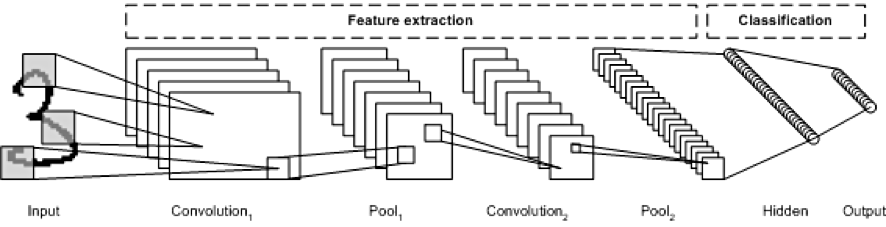
\includegraphics[width=2.5in]{cnn_architecture}
	\caption{An general architecture of the Convolutional Neural Network}
	\label{fig:CNNArchitecture}
\end{figure}

Fig \ref{fig:CNNArchitecture} exhibits an extensive architecture of one CNN with two convolutional operations, two pooling operations, the resulted four groups of feature maps, two fully-connected layers including one hidden layer at the end. It is well known that when designing deep CNN architecture the number of convolutional layers, pooling layers and hidden layers have to be properly defined along with their positions and their configurations. In terms of the configuration, apart from output layer which will always be a number of neurons having the number of classes in the classification problem as the size, different types of layers have different configurations as follows: Filter size, stride size and feature maps are the main attributes of the configurations for convolutional layer; Kernel size, stride size and pooling type - max-pooling or average-pooling are the important fields for the configuration of pooling layers; and the number of neurons is the key attribute of hidden layers. After the layers have been designed, a proper weight initialisation method has to be chosen and in this paper, Xavier weight initialisation \cite{WeightIniti:Glorot} will be chosen as it has been proved as an effective way and has been implemented in most of Deep Learning frameworks.  

\subsection{Particle Swarm Optimisation}

Particle Swarm Optimization (PSO) is a population-based stochastic evolutionary computation algorithm, motivated by the social behaviour of fish schooling or bird flocking \cite{PSOIntro:Kennedy} \cite{PSOIntro:Kennedy}, commonly used for solving optimization problems without rich domain knowledge \cite{PSOIntro:Yanan}. In PSO, the population is comprised of a certain number of particles each of which represent a solution and particles fly in the search space to find the best solution according to Update Equation \ref{eq:UpdateV} and \ref{eq:UpdateX} for velocity and particle vector update respectively where $v_{id}$ represents the velocity, $x_{id}$ represents the particle vector, $P_{id}$ represents the local best of the particle, $P_{gd}$ represents the global best of all the particles, $r_{1}, r_{2}$ are a random number between 0 to 1, $w, c_{1} and c_{2}$ are PSO hyper-parameters used to tweak the performance. 

\begin{equation}\label{eq:UpdateV}
	\begin{aligned}
	v_{id}(t+1) = w * v_{id}(t) + c_{1} * r_{1} * (P_{id} - x_{id}(t)) + \\
	c_{2} * r_{2} * (P_{gd} - x_{id}(t))
	\end{aligned}
\end{equation}

\begin{equation}\label{eq:UpdateX}
	x_{id}(t+1) = x_{id}(t) + v_{id}(t+1)
\end{equation}

\subsection{Internet Protocol address}

An Internet Protocol address (IP address) is a numerical label assigned to each device connected to a computer network that uses the Internet Protocol for communication \cite{IP:Postel}. A network interface contains an IP address to identify the host and its corresponding subnet information used for routing between different networks. A standard IP address widely used is 32-bit number, e.g. 192.168.1.251 and the a standard subnet carries the starting IP address and the length of the subnet mask, e.g. 192.168.1.0/8 which indicates the IP address in the subnet starts from 192.168.1.0 to 192.168.1.255. 

%\subsection{PSO related work in Deep CNN}
%
%As it is shown in Section \ref{sec:CNNArchitecture}, there are a lot of factors that need to be considered when doing the CNN architecture design and it is obviously an extremely hard work for humans to manually achieve the best design. As a result, researchers have been trying to leverage Evolutionary Algorithm to evolve CNN architectures such as LEIC method \cite{LEIC:Real}; However, the learning process is too slow. In this paper, we will design a more efficient PSO method. Since the length of the best CNN architecture on specific problems is not fixed while the particle length of traditional PSO is fixed, the challenge of the proposed PSO method will be inventing a new encoding scheme to cope with the variable-length problem. 

\section{The proposed algorithm}\label{sec:ProposedAlgorithm}
In this section, the IP based PSO (IPPSO) for evolving deep Convolutional Neural Networks for image classification will be documented in details. 


\subsection{Algorithm Overview}
\begin{algorithm}
	\caption{Framework of IP-PSO}
	\label{alg:framework}
	\begin{algorithmic}
		\renewcommand{\algorithmicrequire}{\textbf{Input:}}
		\renewcommand{\algorithmicensure}{\textbf{Output:}}
		\STATE $P \leftarrow$ Initialize the population with the proposed particle encoding strategy
		\STATE $t \leftarrow 0$
		\STATE $P_{id} \leftarrow empty$
		\STATE $P_{gd} \leftarrow empty$
		\WHILE{termination criterion is not satisfied}
			\FOR{$ind$ in $P$}
				\STATE $ind \leftarrow$ update $ind$ using the particle update equation
				\IF{termination criterion is satisfied}
					\STATE $\textbf{break}$
				\ENDIF
			\ENDFOR
		\ENDWHILE		
	\end{algorithmic}
\end{algorithm}

Algorithm \ref{alg:framework} outlines the framework of the proposed algorithm. There are mainly three steps which are really straightforward - initialise the population by using the particle encoding strategy which will be described in Section \ref{sec:ParticleEncodingStrategy}, update the position and velocity and check whether the termination criterion meets.

\subsection{Particle Encoding Strategy}\label{sec:ParticleEncodingStrategy}
IPPSO encoding strategy is derived from the Network IP addresses. Since CNN is comprised of Convolutional Layer, Pooling Layer, and Fully-Connected Layer and the encoded information of different types of layers varies in terms of both the number of fields and the range in each field shown in Table \ref{table:ConvFields} to Table \ref{table:FullFields}, a fixed length of the Network IP with enough capacity can be designed to accommodate all the types of CNN layers and then the Network IP can be divided into numerous subsets each of which can be used to define one type of CNN layers. 

\begin{table}[!t]
	%% increase table row spacing, adjust to taste
	\renewcommand{\arraystretch}{1.3}
	% if using array.sty, it might be a good idea to tweak the value of
	% \extrarowheight as needed to properly center the text within the cells
	\caption{The fields of Convolutional layer with an example in the Example column}
	\label{table:ConvFields}
	\centering
	%% Some packages, such as MDW tools, offer better commands for making tables
	%% than the plain LaTeX2e tabular which is used here.
	\begin{tabular}{|c|c|c|c|}
		\hline
		Field & Example Value & Range & \# of Bits\\
		\hline
		Filter size & 2(001) & 1-8 & 3\\
		\hline
		\# of feature maps & 32(000 1111) & 1-128 & 7\\
		\hline
		Stride size & 2(01) & 1-4 & 2\\
		\hline
		\textbf{Total} & 001 000 1111 01 &  & 12\\
		\hline
	\end{tabular}
\end{table}


\begin{table}[!t]
	%% increase table row spacing, adjust to taste
	\renewcommand{\arraystretch}{1.3}
	% if using array.sty, it might be a good idea to tweak the value of
	% \extrarowheight as needed to properly center the text within the cells
	\caption{The fields of Pooling layer with an example in the Example column}
	\label{table:PoolingFields}
	\centering
	%% Some packages, such as MDW tools, offer better commands for making tables
	%% than the plain LaTeX2e tabular which is used here.
	\begin{tabular}{|c|c|c|c|}
		\hline
		Field & Example Value & Range & \# of Bits\\
		\hline
		Kernel size & 2(01) & 1-4 & 2\\
		\hline
		Stride size & 2(01) & 1-4 & 2\\
		\hline
		Type:1(maximal), 2(average) & 2(1) & 1-2 & 1\\
		\hline
		Place holder & 32(00 1111) & 1-128 & 6\\
		\hline
		\textbf{Total} & 01 01 0 00 1111 &  & 11\\
		\hline
	\end{tabular}
\end{table}

\begin{table}[!t]
	%% increase table row spacing, adjust to taste
	\renewcommand{\arraystretch}{1.3}
	% if using array.sty, it might be a good idea to tweak the value of
	% \extrarowheight as needed to properly center the text within the cells
	\caption{The fields of Fully-Connected layer with an example in the Example column}
	\label{table:FullFields}
	\centering
	%% Some packages, such as MDW tools, offer better commands for making tables
	%% than the plain LaTeX2e tabular which is used here.
	\begin{tabular}{|c|c|c|c|}
		\hline
		Field & Example Value & Range & \# of Bits\\
		\hline
		\# of Neurons & 1024(011 11111111) & 1-2048 & 11\\
		\hline
		\textbf{Total} & 011 11111111 &  & 11\\
		\hline
	\end{tabular}
\end{table}

\begin{table}[!t]
	%% increase table row spacing, adjust to taste
	\renewcommand{\arraystretch}{1.3}
	% if using array.sty, it might be a good idea to tweak the value of
	% \extrarowheight as needed to properly center the text within the cells
	\caption{Disabled layer with an example in the Example column}
	\label{table:DisabledFields}
	\centering
	%% Some packages, such as MDW tools, offer better commands for making tables
	%% than the plain LaTeX2e tabular which is used here.
	\begin{tabular}{|c|c|c|c|}
		\hline
		Field & Example Value & Range & \# of Bits\\
		\hline
		Place holder & 1024(011 11111111) & 1-2048 & 11\\
		\hline
		\textbf{Total} & 011 11111111 &  & 11\\
		\hline
	\end{tabular}
\end{table}

First of all, the length of the IP liked encoding binary string needs to be designed. As the largest number of bits to represent a layer is 12, there will be 2 bytes required to accommodate the 12 bits IP address. 
In addition, the subnets for all types of layers need to be defined and CIDR(Classless Inter-Domain Routing) style will be used to represent the subnet. The subnet 0.0/4 with the range from 0.0 to 15.255 which has the capacity of 12 bits will be used to encode the convolutional layer, the subnet 16.0/5 with the range from 16.0 to 23.255 which has the capacity of 11 bits will represent the fully-connected layer, and the subnet 32.0/5 with the range from 32.0 to 39.255 which has the capacity of 11 bits will carry the information of the Pooling layer. 
Last but not least, as the particle length of PSO is fixed after initialisation,  in order to cope with the variable length of CNN architecture, an alternative way of disabling some of the layers in the encoded particle vector will be used to accomplish it. Therefore another subnet 32.0/5 with the range from 32.0 to 39.255 will be introduced to mark the layer as not used. 
To summarise, the subnet table where the subsets designed to represent the different types of CNN layers can be drawn as Table \ref{table:Subnets} and each layer will be encoded into a 2 bytes IP address. Table \ref{table:IPExample} shows how the example in Table \ref{table:ConvFields} to Table \ref{table:FullFields} is encoded into IP addresses. 

\begin{table}[!t]
	%% increase table row spacing, adjust to taste
	\renewcommand{\arraystretch}{1.3}
	% if using array.sty, it might be a good idea to tweak the value of
	% \extrarowheight as needed to properly center the text within the cells
	\caption{Four subnets distributed to the three types of CNN layers and the disabled layer}
	\label{table:Subnets}
	\centering
	%% Some packages, such as MDW tools, offer better commands for making tables
	%% than the plain LaTeX2e tabular which is used here.
	\begin{tabular}{|c|c|c|}
		\hline
		Layer type & Subnet(CIDR) & IP Range\\
		\hline
		Convolutional Layer & 0.0/4 & 0.0-15.255\\
		\hline
		Fully-Connected Layer & 16.0/5 & 16.0-23.255\\
		\hline
		Pooling Layer & 24.0/5 & 24.0-31.255\\
		\hline
		Disabled Layer & 32.0/5 & 32.0-39.255\\
		\hline
	\end{tabular}
\end{table}

\begin{table}[!t]
	%% increase table row spacing, adjust to taste
	\renewcommand{\arraystretch}{1.3}
	% if using array.sty, it might be a good idea to tweak the value of
	% \extrarowheight as needed to properly center the text within the cells
	\caption{An example of IP addresses - one for each type of CNN layers}
	\label{table:IPExample}
	\centering
	%% Some packages, such as MDW tools, offer better commands for making tables
	%% than the plain LaTeX2e tabular which is used here.
	\begin{tabular}{|c|c|c|}
		\hline
		Layer type & Binary (filled to 2 bytes) & IP address\\
		\hline
		Convolutional Layer & (0000)001 000 1111 01 & 2.61\\
		\hline
		Pooling Layer & (00000)01 01 0 00 1111 & 18.143\\
		\hline
		Fully-Connected Layer & (00000)011 11111111 & 27.255\\
		\hline
		Disabled Layer & (00000)01111111111 & 35.255\\
		\hline
	\end{tabular}
\end{table}

After converting each layer into a 2 bytes IP address, the position and velocity of PSO can be designed. However, there are a few parameters that need to be defined first - max\_length(maximum length of CNN layers), max\_fully\_connected(maximum fully-connected layers with the constraint of at least one fully-connected layer) listed in Table \ref{table:ParameterList}. And then the encoded data type of the position and the velocity will be a byte array with a fixed length of maximum\_length * 2 and each byte will be deemed as one dimension of the particle.

\begin{table}[!t]
	%% increase table row spacing, adjust to taste
	\renewcommand{\arraystretch}{1.3}
	% if using array.sty, it might be a good idea to tweak the value of
	% \extrarowheight as needed to properly center the text within the cells
	\caption{Parameter list}
	\label{table:ParameterList}
	\centering
	%% Some packages, such as MDW tools, offer better commands for making tables
	%% than the plain LaTeX2e tabular which is used here.
	\begin{tabular}{|p{2.5cm}|p{3cm}|p{2cm}|}
		\hline
		Parameter Name & Parameter Meaning & Value\\
		\hline
		max\_length & maximum length of CNN layers & 9\\
		\hline
		max\_fully\_connected & maximum fully-connected layers given at least there is one fully-connected layer & 3\\
		\hline
		N & population size & 30\\
		\hline
		k & the training epoch number before evaluating the trained CNN & 10\\
		\hline
		num\_of\_batch & the batch size for evaluating the CNN & 200\\
		\hline
		c1 & acceleration coefficient array for $P_{id}$ & 1.49618,1.49618\\
		\hline
		c2 & acceleration coefficient array for $P_{gd}$ & 1.49618,1.49618\\
		\hline
		w & inertia weight for updating velocity & 0.7298\\
		\hline
		$v_{max}$ & maximum velocity & 4,25.6(0.1*search space)\\
		\hline
	\end{tabular}
\end{table}

Here is an example of a particle vector to explain how it can cope with variable-length of CNN architecture. Assume we have the parameter settings - max\_length:5, the particle vector could carry a 5-layer CNN such as $[C, C, P, F, F]$ where C represents Conv layer, P represents Pooling layer, F represents fully-connected layer. After a few PSO updates, the vector could turn the fourth element in the vector from F to D to represents a 4-layer CNN such as $[C, C, P, D, F]$ where D means disabled layer. Therefore, the particle is capable to learn a variable-length CNN architecture with the total number of layers less than 5. 

\subsection{Population Initialisation}

\begin{algorithm}
	\caption{Population Initialisation}
	\label{alg:pop_init}
	\begin{algorithmic}
		\renewcommand{\algorithmicrequire}{\textbf{Input:}}
		\renewcommand{\algorithmicensure}{\textbf{Output:}}
		\REQUIRE the population size $N$, the maximum length of CNN layers $max\_length$, the maximum fully-connected layers $max\_fully\_connected$
		\ENSURE Initialised population $P_{0}$
		\STATE $P_{0} \leftarrow$ initialise an empty byte array
		\WHILE{length of $P_{0} < N$}
			\STATE $particle \leftarrow empty$
			\STATE $particle \leftarrow$ Initialise a random IP address in the subnet of convolutional layer and append it to $particle$
			\WHILE{length of $particle < max\_length - max\_fully\_connected \textbf{ AND }$ length of $particle > 0$}
				\STATE $particle \leftarrow$ Initialise a random IP address in a random subnet of convolutional or pooling or disabled layers and append it to $particle$
			\ENDWHILE
			\STATE $is\_fully\_connected\_found \leftarrow \textbf{False}$
			\WHILE {length of $particle > max\_length - max\_fully\_connected \textbf{ AND }$ length of $particle < max\_length-1$}
				\IF{$is\_fully\_connected == \textbf{True}$}
					\STATE $L \leftarrow$ Initialise a random IP address in the subnet of fully-connected layer
				\ELSE
					\STATE $L \leftarrow$ Initialise a random IP address in a random subnet of convolutional or pooling or fully-connected or disabled layers, and set $is\_fully\_connected\_found$ $\textbf{True}$ if the IP represents a fully-connected layer
				\ENDIF
				\STATE $particle \leftarrow$ append $L$ at the end of $particle$ byte array
			\ENDWHILE
			\STATE $paticle \leftarrow$ Initialise a random IP address in the subnet of fully-connected layer and append it to $paticle$
			\STATE $P_{0} \leftarrow$ append $particle$ at the end of $P_{0}$
		\ENDWHILE
		\RETURN $P_{0}$
	\end{algorithmic}
\end{algorithm}

In terms of the population initialisation, as shown in Algorithm \ref{alg:pop_init} we set up the size of the population and randomly create individuals until reaching the population size. 
For each individual, first we initialise an empty vector and each element in it will be used to store a Network Interface containing the IP address and subnet information. The first element will always be a convolutional layer; From the second to (max\_length-max\_fully\_connected) layer each element can be filled with convolutional layer, pooling layer or disabled layer; From (max\_length-max\_fully\_connected) to (max\_length-1) layer it can be filled with any of the four types of layers; And the last element will always be a fully-connected layer. In addition, each layer will be generated with the random settings, a.k.a a random IP address in a specific subnet.


\subsection{Fitness Evaluation}
\begin{algorithm}
	\caption{Fitness Evaluation}
	\label{alg:fitness}
	\begin{algorithmic}
		\renewcommand{\algorithmicrequire}{\textbf{Input:}}
		\renewcommand{\algorithmicensure}{\textbf{Output:}}
		\REQUIRE The population $P_{t}$, the training epoch number $k$, the training set $D_{train}$, the fitness evaluation dataset $D_{fitness}$, the batch size $batch\_size$
		\ENSURE The population with fitness $P_{t}$
		\FOR{individual $s \textbf{ in } P_{t}$}
			\STATE $i \leftarrow 1$
			\WHILE{$i<=k$}
				\STATE $\textit{Train the connection weights of the CNN } \newline \textit{represented by individual s}$
			\ENDWHILE
			\STATE $accy\_list \leftarrow$ Batch-evaluate the trained model on the dataset $D_{fitness}$ with the batch size $batch\_size$ and store the accuracy for each batch
			\STATE ($(mean, stddev) \leftarrow$ Calculate the mean value and standard deviation of  $acc\_list$
			\STATE $num\_of\_connections \leftarrow$ Calculate the number of connections in s
			\STATE $s.fitness \leftarrow (mean, -stddev, -num\_of\_connections)$
		\ENDFOR	
		\RETURN $P_{t}$	
	\end{algorithmic}
\end{algorithm}

With regard to the fitness evaluation in Algorithm \ref{alg:fitness}, each individual is decoded to a CNN with its settings which will be trained for k epoch on the training dataset, and then the trained CNN will be batch-evaluated on the validation dataset which will produce a set of accuracies. Finally, we calculate the mean and standard deviation of the accuracies for each individual which will be stored as the individual fitness along with the number of connections of the CNN. 
For comparing the fitness of individuals, the mean value, standard deviation and the number of parameters will be used in order for the comparison, ie. compare mean value first, if mean value is equal compare standard deviation, if standard deviation is the same compare the number of parameters.


\subsection{Particle Update Equation with Velocity Clamping}
\begin{algorithm}
	\caption{Particle Update Equation with Velocity Clamping}
	\label{alg:update}
	\begin{algorithmic}
		\renewcommand{\algorithmicrequire}{\textbf{Input:}}
		\renewcommand{\algorithmicensure}{\textbf{Output:}}
		\REQUIRE particle individual vector $ind$, acceleration coefficient array for $P_{id}$ $c1$, acceleration coefficient array for $P_{gd}$ $c2$, inertia weight $w$, max velocity array $v_{max}$
		\ENSURE updated individual vector $ind$
		\FOR{element $interface \textbf{ in } ind$}
			\STATE $i \leftarrow 0$
			\FOR{$i <$ number of bytes of IP address in $interface$}
				\STATE $x \leftarrow$ the ith byte of the IP address in the $interface$
				\STATE $(r1, r2) \leftarrow$ uniformly generate $r1, r2$ between [0, 1]
				\STATE $v_{new} \leftarrow$ Update velocity based on PSO update equation: $w * v + c1[i] * r1 * (P_{id} - x) + c2[i] * r2 * (P_{gd} - x)$
				\STATE $v_{new} \leftarrow$ Apply velocity clamping using $v_{max}$
				\STATE $x_{new} \leftarrow x + v_{new}$
				\IF{$x_{new} > 255$}
					\STATE $x_{new} \leftarrow x_{new}-255$
				\ENDIF
			\ENDFOR
		\ENDFOR
		\STATE $fitness \leftarrow$ evaluate the updated individual $ind$
		\STATE $(P_{id}, P_{gd}) \leftarrow$ Update  by comparing them with $fitness$
		\RETURN $ind$
	\end{algorithmic}
\end{algorithm}

In Algorithm \ref{alg:update}, as each layer is encoded into a unit with 2 dimensions in the particle vector and we want to control the acceleration coefficients for each dimension, the two acceleration coefficients are two float arrays with the length of 2. 
After the coefficients defined, we go through each dimension in the individual and update the velocity and position by using the corresponding coefficients for that dimension. Since there are some constraints for each position of the particle vector, e.g. the second element can only be a convolutional layer, pooling layer or disabled layer, we need to upgrade the new position by an interface with a random IP address in a valid subnet if the new position does not fall in a valid subnet. And then we evaluate the new position, compare it with its local best and the global best, and then update the two bests if needed.


\subsection{Best Individual Selection and Decoding}

Global best of PSO will be reported as the best individual. In terms of the decoding, we can first identify the type of the layer represented by the network interface - stored in every 2 bytes/dimensions from left to right in the particle vector of the global best, according to the subnets in Table \ref{table:Subnets} we can distinguish the type of layer, and then based on Table \ref{table:ConvFields} to Table \ref{table:FullFields} we can decode the IP into different sets of bits which indicate different fields of the layer. After decoding all the interfaces in the global best, the final CNN architecture can be obtained by connecting all of the decoded layers in the same order as the interfaces in the particle vector. 

\section{Experiment design}\label{sec:EPDesign}

In order to quantify the performance of the proposed IPPSO for evolving CNN, a series of experiments are designed and performed on the chosen image classification benchmark datasets, which are further compared to state-of-the-art peer competitors. First of all, these benchmark datasets will be briefly described. Secondly, the peer competitors will be listed. Lastly, parameter settings of the proposed IPPSO algorithm participating in these experiments will be documented.

\subsection{Benchmark Datasets}

In these experiments, three datasets are chosen from the widely used image classification benchmark datasets examine the performance of the proposed IPPSO method. They are the MNIST Basic (MB) \cite{DeepArchitectureEval:Larochelle}, the MNIST with Rotated Digits plus Background Images (MRDBI) \cite{DeepArchitectureEval:Larochelle} and the Convex Sets (CS) \cite{DeepArchitectureEval:Larochelle}. 

The first two benchmark datasets are two of the MNIST \cite{DocumentRecognition:LeCun} variants for classifying 10 hand-written digits (i.e., 0-9). There are a couple of reasons for using MNIST variants instead of MNIST. Firstly, the MNIST has been easily achieved 97\%, different noises (e.g., random backgrounds, rotations) are added into these MNIST variants from the MNIST to improve the complexity of classification algorithms. Secondly, there are 12,000 training images and 50,000 test images in these variants, which further challenges the classification algorithms due to the much less training data but more test data. The third benchmark dataset is for recognizing the shapes of objects (i.e., convex or not) which contains 8,000 training images and 50,000 test images. Since it is a two-class classification problem comparing to 10 classes of MNIST dataset and the images contains shapes rather than digits, it is a chosen as a supplement benchmark dataset to the two MNIST variants in order to thoroughly test the performance of the proposed IPPSO method for evolving CNN. 

Each image in these benchmarks is with the size 28 × 28 and examples from these three datasets are displayed in Fig \ref{fig:images}. Another reason for choosing these three benchmark datasets is that different algorithms have reported their promising results, so is convenient for comparing the performance of the proposed IPPSO method with these existing algorithms (details can be seen Subsection \ref{secpeer-competitors}).

\begin{figure}[!t]
	\centering
	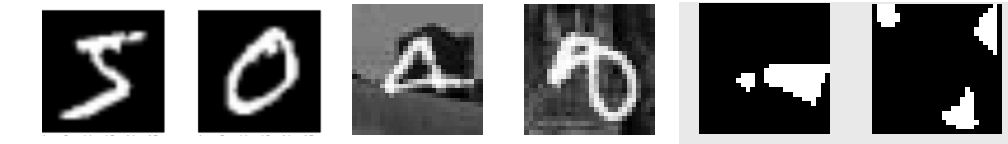
\includegraphics[width=2.5in]{ippso_image_samples}
	\caption{Examples of the three datasets. From left to right, each two images as a group are from one benchmark, and each group is from MB, MRDBI, and Convex, respectively}
	\label{fig:images}
\end{figure}


\subsection{Peer Competitors}\label{secpeer-competitors}

In the experiments, state-of-the-art algorithms that have reported promising classification errors on the chosen benchmarks are collected as the peer competitors of the proposed IPPSO method. To be specific, the peer competitors on the three benchmarks are CAE-2 \cite{CAE:Rifai}, TIRBM \cite{TIRBM:Sohn}, PGBM+DN1 \cite{PGBMDN1:Sohn}, ScatNet-2 \cite{ScatteringCNN:Bruna}, RandNet-2 \cite{DLBaseline:Chan}, PCANet-2 (softmax) \cite{DLBaseline:Chan}, LDANet-2 \cite{DLBaseline:Chan}, SVM+RBF \cite{DeepArchitectureEval:Larochelle}, SVM+Poly \cite{DeepArchitectureEval:Larochelle}, NNet \cite{DeepArchitectureEval:Larochelle}, SAA-3 \cite{DeepArchitectureEval:Larochelle}, and DBN-3 \cite{DeepArchitectureEval:Larochelle}, which are from the literature \cite{DLBaseline:Chan} recently published and the provider of the benchmarks\footnote{\url{http://www.iro.umontreal.ca/∼lisa/twiki/bin/view.cgi/Public/ DeepVsShallowComparisonICML200}}. 

\subsection{Parameter Settings}

All the parameter settings are set based on the conventions in the communities of PSO \cite{PSOEPSettings:Van} and deep learning \cite{DLGuide:Hinton}, in addition to the maximal length of each basic layer which are listed in Table \ref{table:ParameterList}. As both PSO and CNN are involved in the proposed IPPSO method, the parameters can be split into two parts. In regard to CNN parameters, the maximal length of CNN is set to 9 by considering the complexity of the three datasets, the maximal length of fully-connected layer is set to 3 based on the maximal CNN length, the training epoch and the batch size for fitness evaluation is set to 10 and 200 respectively in order not to obtain a CNN architecture that performs well on a specific benchmark dataset in a reasonably short period. In terms of PSO parameters, 30 is used as the population size, 0.7298 is used as the inertia weight, 1.49618 is used as the coefficient of both local best and global best, and 0.1*search\_space, which is (4, 25.6) based on our IP structure design, is used as the maximal velocity for velocity clamping. 

The proposed IPPSO method is implemented in Tensorflow \cite{Tensorfow:Abadi}, and each copy of the code runs on a computer equipped with two GPU cards with the identical model number GTX1080. Due to the heuristic nature of the proposed IPPSO method, 30 independent runs are performed on each benchmark dataset, and the mean results are estimated for the comparisons unless otherwise specified. The experiments take 1 day on each of the benchmark datasets. The source code will be available at https://github.com/wwwbbb8510/ippso for reproducing the experimental results of the proposed IPPSO method reported in this paper, and the evolved CNN architectures on each benchmark are illustrated in Section \ref{sec:EvolvedCNN}.

\section{Experimental results and analysis}\label{sec:EPResults}

In this section, the CNN architectures learned by the proposed IPPSO method from the experiments for the three benchmark datasets will be listed in Section \ref{sec:EvolvedCNN}, and the corresponding classification performance along with the analysis against peer competitors will be shown in Section \ref{sec:Performance}. 

\subsection{Evolved CNN architectures}\label{sec:EvolvedCNN}

Although the proposed IPPSO method is performed on each benchmark with 30 independent runs, only one is chosen on each benchmark for this description that is shown from Table \ref{table:EvolvedMBCNN} to Table \ref{table:EvolvedConvexCNN} because it will be too tedious to list them all and everybody can download and run the code on github. Since disabled layers have been removed during the decoding process, they don't show up in the learned CNN architectures. Therefore, it turns out that IPPSO is able to learn a variable-length CNN architecture which can be obviously seen from the listed architectures - 6 layers for the MB and CONVEX benchmark CNN and 8 layers for the MDRBI benchmark CNN. 

\begin{table}[!t]
	%% increase table row spacing, adjust to taste
	\renewcommand{\arraystretch}{1.3}
	% if using array.sty, it might be a good idea to tweak the value of
	% \extrarowheight as needed to properly center the text within the cells
	\caption{The evolved architecture for the MB benchmark}
	\label{table:EvolvedMBCNN}
	\centering
	%% Some packages, such as MDW tools, offer better commands for making tables
	%% than the plain LaTeX2e tabular which is used here.
	\begin{tabular}{|c|c|}
		\hline
		Layer type & Configuration\\
		\hline
		conv & Filter size: 2, Stride size: 1, feature maps: 26\\
		\hline
		conv & Filter size: 6, Stride size: 3, feature maps: 82\\
		\hline
		conv & Filter size: 8, Stride size: 4, feature maps: 114\\
		\hline
		conv & Filter size: 7, Stride size: 4, feature maps: 107\\
		\hline
		full & Neurons: 1686\\
		\hline
		full & Neurons: 10\\
		\hline
	\end{tabular}
\end{table}

\begin{table}[!t]
	%% increase table row spacing, adjust to taste
	\renewcommand{\arraystretch}{1.3}
	% if using array.sty, it might be a good idea to tweak the value of
	% \extrarowheight as needed to properly center the text within the cells
	\caption{The evolved architecture for the MDRBI benchmark}
	\label{table:EvolvedMDRBICNN}
	\centering
	%% Some packages, such as MDW tools, offer better commands for making tables
	%% than the plain LaTeX2e tabular which is used here.
	\begin{tabular}{|c|c|}
		\hline
		Layer type & Configuration\\
		\hline
		conv & Filter size: 2, Stride size: 1, feature maps: 32\\
		\hline
		conv & Filter size: 6, Stride size: 3, feature maps: 90\\
		\hline
		conv & Filter size: 7, Stride size: 4, feature maps: 101\\
		\hline
		conv & Filter size: 7, Stride size: 4, feature maps: 97\\
		\hline
		pool & Kernel size: 4, Stride size: 4, Type: Average\\
		\hline
		conv & Filter size: 5, Stride size: 3, feature maps: 68\\
		\hline
		full & Neurons: 1577\\
		\hline
		full & Neurons: 10\\
		\hline
	\end{tabular}
\end{table}

\begin{table}[!t]
	%% increase table row spacing, adjust to taste
	\renewcommand{\arraystretch}{1.3}
	% if using array.sty, it might be a good idea to tweak the value of
	% \extrarowheight as needed to properly center the text within the cells
	\caption{The evolved architecture for the CONVEX benchmark}
	\label{table:EvolvedConvexCNN}
	\centering
	%% Some packages, such as MDW tools, offer better commands for making tables
	%% than the plain LaTeX2e tabular which is used here.
	\begin{tabular}{|c|c|}
		\hline
		Layer type & Configuration\\
		\hline
		conv & Filter size: 1, Stride size: 1, feature maps: 11\\
		\hline
		conv & Filter size:7, Stride size: 4, feature maps: 108\\
		\hline
		conv & Filter size: 1, Stride size: 1, feature maps: 8\\
		\hline
		conv & Filter size: 6, Stride size: 3, feature maps: 92\\
		\hline
		full & Neurons: 906\\
		\hline
		full & Neurons: 2\\
		\hline
	\end{tabular}
\end{table}

\subsection{Overall performance}\label{sec:Performance}

Experimental results on all the three benchmark datasets are shown in Table \ref{table:ResultComparison} where the last row denotes the mean classification errors received from the proposed IPPSO method and other rows show the best classification errors reported by peer competitors\footnote{It is a convention in deep learning community that only the best result is reported.}. In order to conveniently investigate the comparisons, the terms “(+)” and “(-)” are provided to indicate whether the result generated by the proposed IPPSO method is better or worse than the best result obtained by the corresponding peer competitor. The term “—” means there is no available result reported from the provider or cannot be counted.

It is clearly shown in Table \ref{table:ResultComparison} that by comparing the result of the proposed IPPSO method with the best performance of the peer competitors it performs the second best on MB dataset which is only a little bit worse than LDANet-2, the best on MDRBI dataset which is the most complicated dataset among these three, and the fifth best on CONVEX dataset which is not ideal but still reasonably competitive. 

\begin{table}[!t]
	%% increase table row spacing, adjust to taste
	\renewcommand{\arraystretch}{1.3}
	% if using array.sty, it might be a good idea to tweak the value of
	% \extrarowheight as needed to properly center the text within the cells
	\caption{The classification errors of the proposed IPPSO method against the peer competitors on the MB, MDRBI and CONVEX benchmark datasets}
	\label{table:ResultComparison}
	\centering
	%% Some packages, such as MDW tools, offer better commands for making tables
	%% than the plain LaTeX2e tabular which is used here.
	\begin{tabular}{|c|c|c|c|}
		\hline
		classifier & MB & MDRBI & CONVEX\\
		\hline
		CAE-2 & 2.48(+) & 45.23(+) & --\\
		\hline
		TIRBM & -- & 35.50(+) & --\\
		\hline
		PGBM+DN-1 & -- & 36.76(+) & --\\
		\hline
		ScatNet-2 & 1.27(+) & 50.48(+) & 6.50(-)\\
		\hline
		RandNet-2 & 1.25(+) & 43.69(+) & 5.45(-)\\
		\hline
		PCANet-2 (softmax)  & 1.40(+) & 35.86(+) & 4.19(-)\\
		\hline
		LDANet-2 & 1.05(-) & 38.54(+) & 7.22(-)\\
		\hline
		SVM+RBF & 3.03(+) & 55.18(+) & 19.13(+)\\
		\hline
		SVM+Poly & 3.69(+) & 56.41(+) & 19.82(+)\\
		\hline
		NNet & 4.69(+) & 62.16(+) & 32.25(+)\\
		\hline
		SAA-3 & 3.46(+) & 51.93(+) & 18.41(+)\\
		\hline
		DBN-3  & 3.11(+) & 47.39(+) & 18.63(+)\\
		\hline
		IPPSO(mean) & 1.15 & 33 & 14\\
		\hline
	\end{tabular}
\end{table}

%\section{Further discussion}\label{sec:FurtherDiscussion}
%
%In this section, we will discuss the two advantages that are brought by the IP structure encoding strategy of the proposed IPPSO method. Other than that an extra finding from the experiments will be pointed out, which could provide insights on the industrial applications of the proposed IPPSO method. 
%
%The first advantage is that the IPPSO method can facilitate the convergence because when the search space is huge, by splitting the search space into several bytes and updating each byte simultaneously which can significantly speed up the learning process. For example, the convolutional layer in our design contains 12 bits and the search space for each dimension in the particle vector will be 4096 if a single decimal is used for the encoding; However, by using the IP-PSO to encode the search space into 2 bytes the search space for each dimension is 256 and PSO can learn them concurrently by updating each of the dimension at every step which can make the convergence much faster. 
%The second advantage is that it provides the flexibility of encoding numerous types of data with variable length into one unit in the particle. For instance, in our design the four types of layers can be encoded as an IP address with 2 bytes which can be easily learned by PSO; However, if using traditional PSO, it is hard to encode 3 types of layers into one number which can be effectively decoded. Furthermore, the capacity of the types of data can extend by enlarging the length of the IP address.
%
%In PSO search process, I found that the architecture learned by only using 1000 rows instead of 12000 rows for MB and MDRBI can obtain a similar or better result than that found by using the whole training set. The potential explanation would be that as we only train the data by 10 epoch and the advantage of using larger data set is to prevent over-fitting which on most occasions will take effect at later training epochs, there is little difference or no difference of using partial dataset instead of the whole dataset which can save a lot of PSO learning time.

% An example of a floating figure using the graphicx package.
% Note that \label must occur AFTER (or within) \caption.
% For figures, \caption should occur after the \includegraphics.
% Note that IEEEtran v1.7 and later has special internal code that
% is designed to preserve the operation of \label within \caption
% even when the captionsoff option is in effect. However, because
% of issues like this, it may be the safest practice to put all your
% \label just after \caption rather than within \caption{}.
%
% Reminder: the "draftcls" or "draftclsnofoot", not "draft", class
% option should be used if it is desired that the figures are to be
% displayed while in draft mode.
%
%\begin{figure}[!t]
%\centering
%\includegraphics[width=2.5in]{myfigure}
% where an .eps filename suffix will be assumed under latex, 
% and a .pdf suffix will be assumed for pdflatex; or what has been declared
% via \DeclareGraphicsExtensions.
%\caption{Simulation results for the network.}
%\label{fig_sim}
%\end{figure}

% Note that the IEEE typically puts floats only at the top, even when this
% results in a large percentage of a column being occupied by floats.


% An example of a double column floating figure using two subfigures.
% (The subfig.sty package must be loaded for this to work.)
% The subfigure \label commands are set within each subfloat command,
% and the \label for the overall figure must come after \caption.
% \hfil is used as a separator to get equal spacing.
% Watch out that the combined width of all the subfigures on a 
% line do not exceed the text width or a line break will occur.
%
%\begin{figure*}[!t]
%\centering
%\subfloat[Case I]{\includegraphics[width=2.5in]{box}%
%\label{fig_first_case}}
%\hfil
%\subfloat[Case II]{\includegraphics[width=2.5in]{box}%
%\label{fig_second_case}}
%\caption{Simulation results for the network.}
%\label{fig_sim}
%\end{figure*}
%
% Note that often IEEE papers with subfigures do not employ subfigure
% captions (using the optional argument to \subfloat[]), but instead will
% reference/describe all of them (a), (b), etc., within the main caption.
% Be aware that for subfig.sty to generate the (a), (b), etc., subfigure
% labels, the optional argument to \subfloat must be present. If a
% subcaption is not desired, just leave its contents blank,
% e.g., \subfloat[].


% An example of a floating table. Note that, for IEEE style tables, the
% \caption command should come BEFORE the table and, given that table
% captions serve much like titles, are usually capitalized except for words
% such as a, an, and, as, at, but, by, for, in, nor, of, on, or, the, to
% and up, which are usually not capitalized unless they are the first or
% last word of the caption. Table text will default to \footnotesize as
% the IEEE normally uses this smaller font for tables.
% The \label must come after \caption as always.
%
%\begin{table}[!t]
%% increase table row spacing, adjust to taste
%\renewcommand{\arraystretch}{1.3}
% if using array.sty, it might be a good idea to tweak the value of
% \extrarowheight as needed to properly center the text within the cells
%\caption{An Example of a Table}
%\label{table_example}
%\centering
%% Some packages, such as MDW tools, offer better commands for making tables
%% than the plain LaTeX2e tabular which is used here.
%\begin{tabular}{|c||c|}
%\hline
%One & Two\\
%\hline
%Three & Four\\
%\hline
%\end{tabular}
%\end{table}


% Note that the IEEE does not put floats in the very first column
% - or typically anywhere on the first page for that matter. Also,
% in-text middle ("here") positioning is typically not used, but it
% is allowed and encouraged for Computer Society conferences (but
% not Computer Society journals). Most IEEE journals/conferences use
% top floats exclusively. 
% Note that, LaTeX2e, unlike IEEE journals/conferences, places
% footnotes above bottom floats. This can be corrected via the
% \fnbelowfloat command of the stfloats package.




\section{Conclusion and future work}\label{sec:Conclusion}

The goal of this paper was to develop a new PSO approach with variable length to automatically evolve the architectures of CNNs for image classification problems. This goal has been successfully achieved by proposing a new encoding scheme of using a network interface containing an IP address and its corresponding subnet to carry the configurations of a CNN layers, a corresponding decoding method to translate a network interface back to a CNN layer, a series of three subnets to represent three types of CNN layers, an additional subnet for disabling some dimensions in the particle vector in order to achieve a variable-length PSO, a new update equation with velocity clamping specifically for the proposed encoding scheme, and an efficient fitness evaluation method. This approach was examined and compared with 12 peer competitors including the most state-of-the-art algorithms on three benchmark datasets commonly used in deep learning and the experiment results show that the proposed IPPSO method can achieve a very competitive accuracy by outperforming all others on the MDRBI benchmark dataset, being the second-best on the MNIST benchmark dataset and ranking above the middle on the CONVEX benchmark dataset. 

The most important improvement from PSO to the novel IPPSO proposed in the paper is to invent the new encoding strategy of using network interface. Since the subnet in the interface can distinguish any type of layers, any layer configurations can be encoded into the IP address and the length of the IP address can be easily extended to 4 bytes (the length of real IP addresses) or even more, the IPPSO method has the ability of encoding any type of Deep Neural Network layers. In addition, the particle length of the IPPSO method can be easily made variable by simply introducing a disabled layer which could be deemed crucial as it breaks the obstacle of traditional PSO being fix-length. 

In this paper, we have investigated the proposed IPPSO method for evolving deep CNN and it is proved of obtaining promising results. Based on this research, there are a couple of further researches that are worth doing. Firstly, as this paper is mainly to propose the novel encoding strategy of the IPPSO, it will be interesting to see how different PSO topologies\footnote{Fully-connected topology is used in this paper as it is easy to be implemented} will affect the performance of the IPPSO and find the best topology for it. Secondly, we will also investigate how the proposed IPPSO algorithm performs for evolving recurrent neural networks, which are powerful tools for addressing sequential data, such as language processing problem.

% conference papers do not normally have an appendix


% use section* for acknowledgment
%\section*{Acknowledgement}


%The authors would like to thank all the supervisors. 





% trigger a \newpage just before the given reference
% number - used to balance the columns on the last page
% adjust value as needed - may need to be readjusted if
% the document is modified later
%\IEEEtriggeratref{8}
% The "triggered" command can be changed if desired:
%\IEEEtriggercmd{\enlargethispage{-5in}}

% references section

% can use a bibliography generated by BibTeX as a .bbl file
% BibTeX documentation can be easily obtained at:
% http://mirror.ctan.org/biblio/bibtex/contrib/doc/
% The IEEEtran BibTeX style support page is at:
% http://www.michaelshell.org/tex/ieeetran/bibtex/
%\bibliographystyle{IEEEtran}
% argument is your BibTeX string definitions and bibliography database(s)
%\bibliography{IEEEabrv,../bib/paper}
%
% <OR> manually copy in the resultant .bbl file
% set second argument of \begin to the number of references
% (used to reserve space for the reference number labels box)
\begin{thebibliography}{}

\bibitem{EvolveCNN:Yanan}
Yanan Sun, Bing Xue, Mengjie Zhang, \emph{Evolving Deep Convolutional Neural Networks for Image Classification[J]}. arXiv preprint arXiv:1710.10741, 2017. 

\bibitem{EvolveDNN:Yanan}
Yanan Sun, Gary G. Yen, Zhang Yi, \emph{Evolving Unsupervised Deep Neural Networks for Learning Meaningful Representations[J]}. arXiv preprint arXiv:1712.05043, 2017. 

\bibitem{PSOIntro:Yanan}
Yanan Sun, Bing Xue, Mengjie Zhang, \emph{A Particle Swarm Optimization-based Flexible Convolutional Auto-Encoder for Image Classification[J]}. arXiv preprint arXiv:11712.05042, 2017. 

\bibitem{PSOIntro:Kennedy}
Kennedy and R. E. P. S. Optimization, \emph{Ieee int,} in Conf. on Neural Networks, vol. 4, 1995

\bibitem{PSOIntro:Eberhart}
. Eberhart and J. Kennedy, \emph{A new optimizer using particle swarm theory}, in Micro Machine and Human Science, 1995. MHS’95., Proceedings of the Sixth International Symposium on.  IEEE, 1995, pp. 39–43.

\bibitem{IP:Postel}
Postel, J., \emph{DoD standard Internet Protocol}, RFC 760, DOI 10.17487/RFC0760, January 1980, <https://www.rfc-editor.org/info/rfc760>.

\bibitem{CNNspeech:Ossama}
Ossama Abdel-Hamid, Li Deng and Dong Yu, \emph{Exploring Convolutional Neural Network Structures and Optimization Techniques for Speech Recognition}. INTERSPEECH 2013, 5 - 29 August 2013, Lyon, France

\bibitem{CNNsentence:Yoon}
Yoon Kim, \emph{Convolutional Neural Networks for Sentence Classification}, arXiv:1408.5882v2 [cs.CL] 3 Sep 2014

\bibitem{ImageNet:Alex}
Alex Krizhevsky, Ilya Sutskever and Geoffrey E. Hinton, \emph{ImageNet Classification with Deep Convolutional Neural Networks}, Advances in Neural Information Processing Systems 25 (NIPS 2012), 2012

\bibitem{ZipcodeRecognition:LeCun}
Y. LeCun, B. Boser, J. S. Denker, D. Henderson, R. E. Howard, W. Hubbard, and L. D. Jackel, \emph{Backpropagation applied to handwritten zip code recognition}, Neural Computation, vol. 1, no. 4, pp. 541–551, 1989. 

\bibitem{DocumentRecognition:LeCun}
Y. LeCun, L. Bottou, Y. Bengio, and P. Haffner, \emph{Gradient-based learning applied to document recognition}, Proceedings of the IEEE, vol. 86, no. 11, pp. 2278–2324, 1998.

\bibitem{CNNverydeep:Simonyan}
K. Simonyan and A. Zisserman, \emph{Very deep convolutional networks for large-scale image recognition}, arXiv preprint arXiv:1409.1556, 2014.

\bibitem{CNNdeeper:Szegedy}
C. Szegedy, W. Liu, Y. Jia, P. Sermanet, S. Reed, D. Anguelov, D. Erhan, V. Vanhoucke, and A. Rabinovich, \emph{Going deeper with convolutions,” in Proceedings of the IEEE Conference on Computer Vision and Pattern Recognition}, 2015, pp. 1–9.

\bibitem{CNNGP:Suganuma}
Masanori Suganuma, Shinichi Shirakawa, and Tomoharu Nagao, \emph{A Genetic Programming Approach to Designing Convolutional Neural Network Architectures∗}, arXiv:1704.00764v2  [cs.NE]  11 Aug 2017

\bibitem{CNNevolve:Stanley}
K. O. Stanley and R. Miikkulainen, \emph{Evolving neural networks through augmenting topologies}, Evolutionary computation, vol. 10, no. 2, pp. 99–127, 2002.

\bibitem{FashionImage:Xiao}
H. Xiao, K. Rasul, and R. Vollgraf, \emph{Fashion-mnist: a novel image dataset for benchmarking machine learning algorithms}, arXiv preprint arXiv:1708.07747, 2017.

\bibitem{DeepArchitectureEval:Larochelle}
H. Larochelle, D. Erhan, A. Courville, J. Bergstra, and Y. Bengio, \emph{An empirical evaluation of deep architectures on problems with many factors of variation}, in Proceedings of the 24th International Conference on Machine Learning. ACM, 2007, pp. 473–480.

\bibitem{CAE:Rifai}
S. Rifai, P. Vincent, X. Muller, X. Glorot, and Y. Bengio, \emph{Contractive auto-encoders: Explicit invariance during feature extraction}, in Proceedings of the 28th International Conference on Machine Learning, 2011, pp. 833–840. 

\bibitem{TIRBM:Sohn}
K. Sohn and H. Lee, \emph{Learning invariant representations with local transformations}, arXiv preprint arXiv:1206.6418, 2012. 

\bibitem{PGBMDN1:Sohn}
K. Sohn, G. Zhou, C. Lee, and H. Lee, \emph{Learning and selecting features jointly with point-wise gated boltzmann machines}, in International Conference on Machine Learning, 2013, pp. 217–225. 

\bibitem{DLBaseline:Chan}
T.-H. Chan, K. Jia, S. Gao, J. Lu, Z. Zeng, and Y. Ma, \emph{Pcanet: A simple deep learning baseline for image classification?} IEEE Transactions on Image Processing, vol. 24, no. 12, pp. 5017–5032, 2015. 

\bibitem{ScatteringCNN:Bruna}
J. Bruna and S. Mallat, \emph{Invariant scattering convolution networks}, IEEE transactions on Pattern Analysis and Machine Intelligence, vol. 35, no. 8, pp. 1872–1886, 2013. 

\bibitem{PSOEPSettings:Van}
F. van den Bergh, A.P. Engelbrecht, \emph{A study of particle swarm optimization particle trajectories}, doi:10.1016/j.ins.2005.02.003

\bibitem{DLGuide:Hinton}
G. E. Hinton, \emph{A practical guide to training restricted boltzmann machines}, in Neural Networks: Tricks of the Trade. Springer, 2012, pp. 599–619.

\bibitem{Tensorfow:Abadi}
M. Abadi, A. Agarwal, P. Barham, E. Brevdo, Z. Chen, C. Citro, G. S. Corrado, A. Davis, J. Dean, M. Devin et al., \emph{Tensorflow: Large-scale machine learning on heterogeneous distributed systems}, arXiv preprint arXiv:1603.04467, 2016. 

\bibitem{PSO:OptimiseCNN}
Arie Rachmad Syulistyo, Dwi M J Purnomo, Muhammad Febrian Rachmadi, and Adi Wibowo, \emph{Particle swarm optimization (PSO) for training optimization on convolutional neural network (CNN) }, Jurnal Ilmu Komputer dan Informasi (Journal of Computer Science and Information). 9/1 (2016), 52-58 DOI: http://dx.doi.org/10.21609/jiki.v9i1.366

\bibitem{WeightIniti:Glorot}
X. Glorot and Y. Bengio, \emph{Understanding the difficulty of training deep feedforward neural networks}, in Proceedings of the 13th International Conference on Artificial Intelligence and Statistics, 2010, pp. 249–256. 

\bibitem{LEIC:Real}
E. Real, S. Moore, A. Selle, S. Saxena, Y. L. Suematsu, Q. Le, and A. Kurakin, “Large-scale evolution of image classifiers,” arXiv preprint arXiv:1703.01041, 2017. 

\end{thebibliography}




% that's all folks
\end{document}


